\section{Recap: Probability and Statistics}
\subsection{Probability Space} 
Our intuitive notion of probability is related to uncertainty we have about events in the world, for example - will it rain tomorrow? How much will I get in the final exam? Although we cannot predict with certainty the answers to these questions, we usually know what is the set of all possible outcomes. This gives us the first ingredient in any \emph{probability space}.
\footnote{This section is based on lecture notes by Michal Moshkovitz and Alon Gonen}
\begin{definition}
A \emph{sample space} $\Omega$ is a set that contains all possible outcomes. $\omega\in\Omega$ denotes a single outcome.
\end{definition}
Examples:
\begin{itemize}
\item Coin toss: $\Omega=\left\{ H,T\right\} $
\item Toss a coin until heads comes up: $\Omega=\left\{ T^{n-1}H:n\in\mathbb{N}_0\right\} $
\item Rolling two dice: $\Omega=\left\{ 1,\dots,6\right\} ^{2}$
\item Waiting time at the post office: $\Omega=[0,\infty)$
\end{itemize}
Suppose someone threw a die (singular of dice), and told us that the result is an even number. This result is not an element in $\Omega$, but it tells us that the outcome is an element in the subset $\left\{ 2,4,6\right\} $.
\begin{definition}
An \emph{event} $A$ is any subset of possible outcomes, $A\subseteq\Omega$.
\end{definition}
Quick reminder:
\begin{itemize}
\item $A^{c}$ (or sometimes $\overline{A}$) denotes the \textit{complement} of $A$, $A^{c}=\Omega\backslash A$ . In other words, $A^{c}$ is the event that $A$ did not occur.
\item We say that $A$ and $B$ are \textit{disjoint events} if $A\cap B=\emptyset$.
\item $\Omega$ and $\emptyset$ are also events. If $A$ and $B$ are two events, then $A\cup B$ is also an event, and so is $A\cap B$.
\end{itemize}

Intuitively, a probability function assigns to an event a number which quantifies our knowledge or belief about the possibility of observing any outcome in that event.


%\subsubsection*{Discrete models }
\begin{definition}
A \emph{probability space} is a tuple \footnote{For our needs this simple and intuitive definition is sufficient, though, richer definitions exist.} $(\Omega, \cD)$ where $\Omega$ is a \emph{sample space} and $\cD:2^{\Omega}\rightarrow\reals$ is a probability function such that
\begin{enumerate}
\item $\cD(\Omega)=1$
\item for all $\omega\in\Omega, \cD(\omega)\in[0,1]$
\item for all $A,B\subseteq\Omega$ such that $A\cap B=\emptyset,$ we have $\cD(A \cup B)=\cD(A)+\cD(B).$
\end{enumerate}
\end{definition}
%\begin{exercise} Find he probability space that corresponds to a fair coin toss.
%\end{exercise}
%Solution: $\Omega=\{H,T\},\Pr(H)=\Pr(T)=0.5$
\begin{example}
Suppose we throw two fair dice, then $\Omega=\left\{ 1,\dots,6\right\} ^{2}$ and $\cD\left(\left(i,j\right)\right)=\frac{1}{36}$
\end{example}

\begin{exercise}
For all $A,B\subseteq\Omega$: $\cD(A\cup B)=\cD(A)+\cD(B)-\cD(A\cap B)$
\end{exercise}
Solution:\\
$A\cup B=(A\setminus B)\cup(B\setminus A)\cup(A\cap B)\; ,A=(A\setminus B)\cup(A\cap B)$ and $B=(B\setminus A)\cup(A\cap B).$
$$\cD(A\cup B)=\cD(A\setminus B)+\cD(B\setminus A)+\cD(A\cap B)=\cD(A)-\cD(A\cap B)+\cD(B) - \cancel{\cD(A\cap B)}  + \cancel{\cD(A\cap B)} $$

\begin{definition}
$A,B\subseteq\Omega$ are called \emph{independent} if the occurrence of one does not affect the probability of occurrence of the other. Consequently: $$\cD(A\cap B) =\cD(A)\cdot\cD(B).$$
\end{definition}

\begin{exercise}
If $A$ and $B$ are independent then $A$ and $B^c$ are also independent.
\end{exercise}
Solution: $\cD(A)=\cD(A\cap B)+\cD(A\cap B^c)\Rightarrow\cD(A\cap B^c)=\cD(A)(1-\cD(B))=\cD(A)\cdot\cD(B^c).$\\


\begin{lemma}  \label{lem:unionBound}  \textbf{(The union bound)} Let
$(\Omega, \cD)$ be a probability space. The probability function is \emph{sub-additive}, i.e., for any sequence $(A_k)$ of events,
\[
\cD(\cup_{k=1}^\infty A_k) \le \sum_{k=1} ^\infty \cD(A_k)
\]
\end{lemma}
\begin{proof}
Let $B_1=A_1$. For each $k \in \{2,3,\ldots\}$, let $B_k = A_k
\setminus \cup_{i=1}^{k-1} A_i$. Note that the $B_1...B_k$ are disjoint, and
$\cup_{i=1}^k A_i=\cup_{i=1}^k B_i$. Also, since $B_k\subseteq A_k$, $\cD(B_k) \le \cD(A_k)$ for every $k \in \bN$. It follows by the countable additivity of $\cD$ that
\[
\cD(\cup_{k=1}^\infty A_k) = \cD(\cup_{k=1}^\infty B_k) = \sum_{k=1}
^\infty \cD(B_k) \le \sum_{k=1}
^\infty \cD(A_k)~.
\]
\end{proof}




\subsection{Random Variables, discrete and continuous}

So far we have asked questions like: does an event happen or not and what is the probability of the event. But what about different questions- such as  "how much." For example, if we get a dollar if a coin flip turns head, we can ask how many dollars would we get after 3 rounds? \\

In order to answer this question, we should understand the sample space, which is
 $\Omega=\{HHH,HHT,HTH,THH,HTT,THT,TTH,TTT\}$. Then we would need to define a reward function that will quantify ones's profit for each outcome of the experiment ($\omega\in \Omega$):
 $M(HHH)=3,M(HHT)=2.$ This quantifying function $M$ is called a \emph{random variable} (RV).
\begin{definition}
Given a probability space $\left(\Omega,\cD\right)$, a real-valued \emph{random variable (RV)} is a function $X:\Omega\rightarrow\mathbb{R}$.

\end{definition}
\begin{remark}
Any function $g\left(X\right)$ of a random variable is also a random
variable (for instance $X^{2}$, $\sgn \left(X\right)$, etc.).
\end{remark}
For a discrete $\Omega$ we define the \textbf{\textit{probability
mass function (PMF)}} of $X$ (a \textit{discrete RV}) as
\[
\cD\left(\left\{ X=x\right\} \right)=\sum_{\omega:X\left(\omega\right)=x}\cD\left(\omega\right)
\]


Instead of writing $\cD\left(\left\{ X=x\right\} \right)$ we usually
write $\cD\left(x\right)$.

\begin{example}
A fair coin is tossed twice. The probability space is given by $\Omega=\left\{ T,H\right\} ^{2}$
and  $\cD\left(\omega\right)=\frac{1}{4}$ for any $\omega\in \Omega$. Let $X$ denote the number of heads obtained in each outcome ($\omega$). The image of $X$ is  $\mathcal{X}=\left\{ 0,1,2\right\} $
and
\[
\cD\left(x\right)=\begin{cases}
\frac{1}{4} & x=0,2\\
\frac{1}{2} & x=1\\
0 & \mbox{else}
\end{cases}
\]

\end{example}


For a continuous $\Omega$ - we say that $X$ is a \textit{continuous
RV} if there exists $f(x)\ge 0$ so that we can write, for every $D\subset\mathbb{R}$
\[
\cD\left(X\in D\right)=\int_{D}f\left(x\right)dx
\]


In particular, this means that for any $a,b\in \mathbb{R}$, where $a\leq b$:
\[
\cD\left(X\in\left[a,b\right]\right)=\int_{a}^{b}f\left(x\right)dx
\]

In this course we assume that $f(x)$ is a regular function and therefore the probability mass function for a single point is 0: $\cD\left(X=a\right)=\int_{a}^{a}f\left(x\right)dx=0$ for any $a\in\mathbb{R}$.

The function $f$ is called the \textbf{\textit{probability density
function }}\textbf{(PDF)} of $X$. Note that -
\begin{itemize}
\item $f\left(x\right)\ge0$
\item $\int_{-\infty}^{\infty}f\left(x\right)dx=1$
\item $f\left(x\right)$ is a probability \emph{density}, not a probability. For example, it could be that $f\left(x\right)>1$.\\
\end{itemize}

\subsection{Mean and Variance}
\begin{definition}
The \textbf{\textit{expected value}} of a random variable
$X$ is
\[
\bE\left[X\right]=\sum_{x\in\mathcal{X}}x\cD\left(x\right)\qquad\mbox{or}\qquad \bE\left[X\right]=\int_{-\infty}^{\infty}xf\left(x\right)dx
\]

\end{definition}
Properties:
\begin{itemize}
\item $\bE\left[g\left(X\right)\right]=\sum g\left(x\right)\cD\left(x\right)$,
\item $\bE\left[c\right]=c$
\item Linear: $\bE\left[aX+Y\right]=a\bE\left[X\right]+\bE\left[Y\right]$
\item If $X$ and $Y$ are independent then $\bE\left[XY\right]=\bE\left[X\right]\bE\left[Y\right]$
(explanation: $\bE[XY]=\sum\cD(X=x,Y=y)x\cdot y = \sum_{x,y}\cD(x)\cD(y)xy=\bE[X]\bE[Y]$)
\end{itemize}

\begin{definition}
Let $X$ be a RV with $\bE\left[X\right]=\mu$, then the \textbf{\textit{variance}}
of $X$ is
\[
V\left(X\right)=\bE\left[\left(X-\mu\right)^{2}\right]
\]
The \textbf{\textit{standard deviation}} is defined as $\sigma=\sqrt{V\left(X\right)}$.
\end{definition}
Properties of the variance:
\begin{itemize}
\item $V(X)\geq0$ , ~$V(X)=0\,\iff\,X$ is a constant.
\item $V\left(X\right)=\bE\left[X^{2}\right] - (\bE\left[X\right])^{2}$
\item $V(aX+b)=a^{2}V(X)$
\item $V(X+Y)=\bE\left[\left(X+Y-\bE(X)-\bE(Y)\right)^{2}\right]=V(X)+V(Y)+2\overbrace{\bE\left[\left(X-\bE[X]\right)\left(Y-\bE[Y]\right)\right]}^{\cov\left(X,Y\right)}$
\item If $X_{1},\dots,X_{n}$ are independent then $V\left(\sum X_{i}\right)=\sum V\left(X_{i}\right)$\end{itemize}

\begin{definition}
The \textbf{\textit{covariance}} of $X$ and $Y$ is
\end{definition}
\[
\cov(X,Y)=\bE\left[\left(X-\bE[X]\right)\left(Y-\bE[Y]\right)\right]=\bE\left[XY\right]-\bE[X]\bE[Y]
\]

Properties:
\begin{itemize}
\item $\cov(X,Y)=\cov(Y,X)$
\item $\cov(aX+b,cY+d) = a \cdot c \cdot \cov(X,Y)$
\item $\cov(X,X)=V(X)$
\end{itemize}
%We say that $X$ and $Y$ are \textbf{\emph{uncorrelated}}\emph{ }\textit{\emph{if $\cov\left(X,Y\right)=0$.}}
%\begin{remark}
%If $X$ and $Y$ are uncorrelated it does not imply that they are independent.\end{remark}

\begin{exercise}
Let $Z$ be a Bernoulli random variable. Calculate $Var[Z].$
\end{exercise}
Solution: $Var[Z] = \bE[Z^2] - (\bE[Z])^2 = p-p^2=p(1-p).$


\begin{example}
Find the mean and variance of $X\sim U\left(\left[a,b\right]\right),$ where $U[a,b]$ is the uniform distribution on $[a,b].$
\begin{eqnarray*}
\bE\left[X\right] & = & \frac{1}{b-a}\int_{a}^{b}xdx=\frac{1}{2\left(b-a\right)}\left(b^{2}-a^{2}\right)=\frac{b+a}{2}\\
\bE\left[X^{2}\right] & = & \frac{1}{b-a}\int_{a}^{b}x^{2}dx=\frac{1}{3\left(b-a\right)}\left(b^{3}-a^{3}\right)=\frac{b^{2}+ab+a^{2}}{3}\\
V\left(X\right) & = & \frac{b^{2}+ab+a^{2}}{3}-\frac{\left(b+a\right)^{2}}{4}=\frac{\left(b-a\right)^{2}}{12}
\end{eqnarray*}
\end{example}

\subsection{A little Statistics: Mean and variance estimation}

This is a course in {\em Statistical} Machine Learning. So let's start with a little bit of statistics. Some of you may have never seen statistics before. 
When we study {\em Probability} we assume a known distribution and calculate probability of events of interest. When we we study {\em Statistics} we turn the question on its head: using samples from an unknown probability distribution, we try to {\em estimate} or {\em test} properties of of the unknown distribution. 

Take the mean and variance of a probability distribution for example. 
The mean gives us a taste of around which point the data is distributed. The variance on the other hand gives you a taste of the concentration of the "spread" of the distribution around its mean. 
Low variance usually means that the distribution is highly concentrated around the mean, while high variance means that the distribution is less concentrated there.\\
In a probability course, given that we know the distribution, we learned how to calculate its mean and variance. 
Now we would like to ask a different question. We are given {\em samples} that were drawn from an unkown distribution.
Can we {\em estimate}  the distribution's mean and variance using only those samples?\\

Formally, let $X$ be a random variable, let $p_X$ be its (unknown) distribution, and let $X_1,\ldots,X_n\overset{i.i.d}{\sim} p_X$.
Here, i.i.d  denotes \emph{independent and identically distributed} random variables. We are given \emph{data}
samples: $x_1,\ldots,x_n$, where $x_i$ is a {\em number} - the sample obtained by sampling $X_i$.
In statistics, $\bE[X]$ is called the {\em population} mean and  $V(X)$ is called the population variance. 
So, what is a "reasonable" \textbf{estimator} for $\bE[X]$ and $V(X)$ based only on those $n$ samples?\\

Throughout the course we are going to use the following estimators (commonly denoted with the "hat" symbol $\hat{\circ}$):
\begin{itemize}
    \item Sample mean (an estimator for the population mean)
    \begin{eqnarray*}
    \hat{\mu}_X = \frac{1}{n} \sum_{i=1}^n x_i
    \end{eqnarray*}
    \item Sample variance (an estimator for population variance)
    \begin{eqnarray*}
    \hat{\sigma}_X^2 = \frac{1}{n-1} \sum_{i=1}^n (x_i-\hat{\mu}_X)^2
    \end{eqnarray*}
    % It is important to note that if you do know the mean of the data, then the sample variance will look like that:
    % \begin{eqnarray*}
    % \hat{\sigma}_X^2 = \frac{1}{n} \sum_{i=1}^n (x_i-\mu)^2
    % \end{eqnarray*}
\end{itemize}
{Note the $\frac{1}{n-1}$ factor. Why not use $\hat{\Sigma}_X^2 = \frac{1}{n} \sum_{i=1}^n (x_i-\hat{\mu}_X)^2$ as the variance estimator? \emph{Answer}: calculate the expected value of these estimators and you will find (perhaps surprisingly) that $\bE[\hat{\sigma}_X^2]=V(X)$ while $\bE[\hat{\Sigma}_X^2] = \frac{n-1}{n}V(X)$. So, in expectation, $\hat{\sigma}_X^2$ gets the population variance exactly. When an estimator for some parameter of the unknown distribution gets the desired parameter exactly {\em in expectation}, we call that estimator {\em unbiased} for that parameter. 


We invite you to read some additional material about the sample variance and the population variance {\color{blue}\href{https://www.macroption.com/population-sample-variance-standard-deviation/}{\textbf{here}}}  and {\color{blue}\href{https://en.wikipedia.org/wiki/Bias_of_an_estimator}{\textbf{here}}} if you want to understand the reason for the difference in the formula. \\

\section{High dimensional distributions}
Back to probability. Now, instead of random variables that take real (scalar) value,  we will consider a more general case in which they take vector values in $\reals^d$, where $d\in \bN$.

\subsection{Basic definitions}

\begin{definition}[Random vector]
A finite collection of random variables, denoted $X_1, \dots, X_n$ (defined on a common probability space $(\Omega, \cD)$) is a random (column) vector: $\boldsymbol{X} = (X_1, \dots, X_n)^T$

\end{definition}


\begin{definition}[Joint distribution]
Given random variables $X_1, \dots, X_n$ , that are defined on a probability space, the joint probability distribution for $X_1, \dots, X_n$ is a probability distribution that gives the probability that each of $X_1, \dots, X_n$ falls in any particular range (for continuous RVs) or discrete set (for discrete RVs) of values specified for that variable.

\end{definition}


\begin{definition}[Joint PDF of a random vector]
Two random variables $X$ and $Y$ are jointly continuous if there exists a nonnegative function $f_{XY}: \reals^2 \to \reals$, such that, for any set $A \in \reals^2$, we have
$$
\cD\left( (X,Y) \in A \right) = \int_A f_{XY}(x, y) dx dy
$$
The function $f_{XY}(x, y)$ is called the \emph{joint probability density function (JPDF)} of $X$ and $Y$.
This can of course be generalized to any dimension. 

\end{definition}

\begin{remark}[PDF for a random vector]
Given $\boldsymbol{X} = (X_1, \dots, X_n)^T$, each of the scalar random variables $X_1, \dots, X_n$ can be characterized by its PDF. However, unless the scalar RV's are mutually independent, the PDF of each coordinate of a random vector does not completely describe the probabilistic behaviour of the whole vector. For instance, $X_1$ and $X_2$ could have the same PDF, but still the behavior of $\boldsymbol{X} = (X_1, X_2)$ and $\boldsymbol{\Tilde{X}} = (X_1, X_1)$ can be drastically different. For example, consider $X_1 \sim U([-a, a])$ and $X_2 = - X_1$. 

\end{remark}



\subsection{Normal Distribution}
As an example of random vectors, we now consider specific family of distributions- the Multivariate Normal (or Multivariate Gaussian) Distributions. The normal distribution is very useful for many reasons. One reason is the Central Limit Theorem (CLT). You have likely seen the one-dimensional ("univariate") version of the CLT in your probability course. In one of its forms, under some conditions, the CLT states that sample mean of random i.i.d variables (when properly scaled) converges in distribution to the normal distribution. There is a multivariate version of the CLT, which is one reason why you want to be familiar with the multivariate normal distribution. Another reason we like the (multivariate) normal distribution is that many results and methods (such as propagation of uncertainty and least squares parameter fitting) can be derived analytically in explicit form when the relevant variables are (multivariate) normally distributed.

\begin{definition}[Univariate Normal Distribution (namely, in dimension $d=1$)] \label{def: UVN}
A random variable x has a normal distribution with expectation $\mu$ and variance $\sigma^2$ if it has a PDF of the form:
$$f(x) = \frac{1}{\sqrt{2\pi\sigma^2} } e^{ -\frac{(x-\mu)^2}{2\sigma^2} } $$
In this case we write: $x\sim\mathcal{N}({\mu},{\sigma^2})$

\end{definition}
\begin{definition}[Multivariate Normal Distribution] \label{def: MVN}
random vector x has a multivariate normal distribution with expectation $\mu$ and covariance matrix (see definition below) $\Sigma$ if it has a joint PDF of the form:
$$f\left(x\right)=\frac{1}{\sqrt{\left(2\pi\right)^{n}\left|\Sigma\right|}}\exp\left\{ -\frac{\left(x-\mu\right)^{T}\Sigma^{-1}\left(x-\mu\right)}{2}\right\} $$
In this case we write: $x\sim\mathcal{N}(\boldsymbol{\mu},\boldsymbol{\Sigma})$
\end{definition}

\begin{figure}[h!]
  \centering
  \begin{minipage}[b]{0.4\textwidth}
        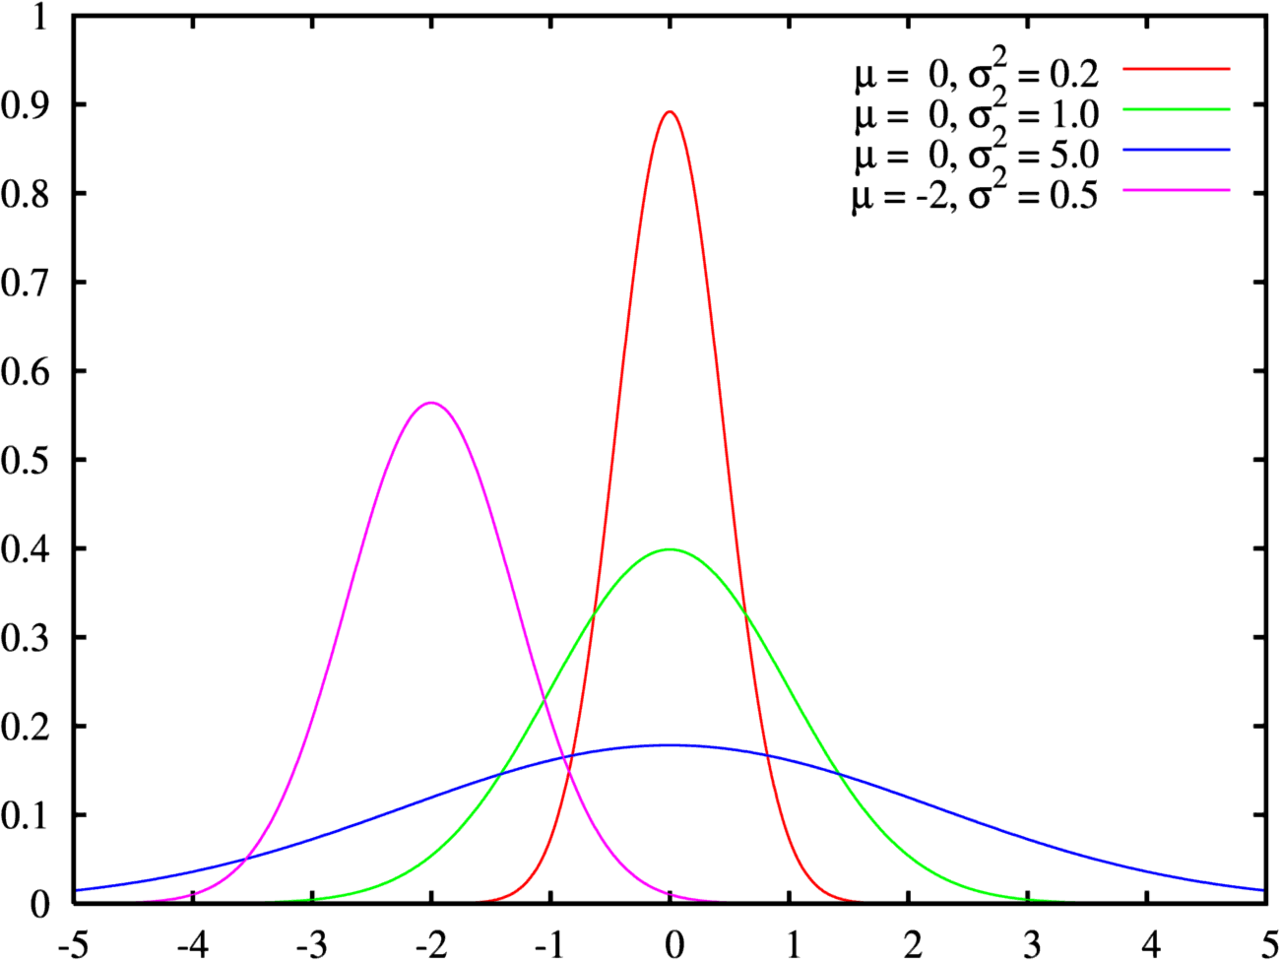
\includegraphics[scale=0.1]{1D.png}
   \caption{$f(x) = \frac{1}{\sqrt{2\pi\sigma^2} } e^{ -\frac{(x-\mu)^2}{2\sigma^2} } $}
  \end{minipage}
  \hfill
  \begin{minipage}[b]{0.5\textwidth}
       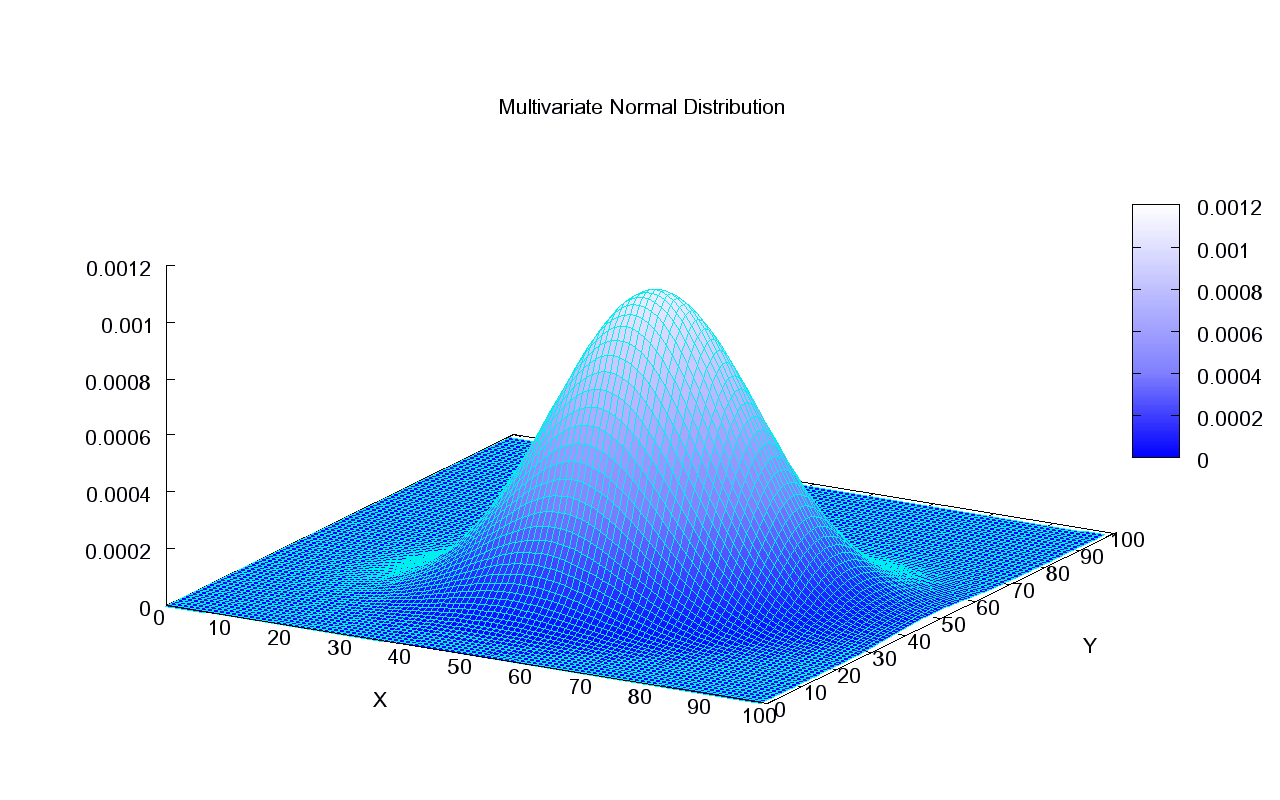
\includegraphics[scale=0.1]{2D.png}
   \caption{
   \begingroup
\footnotesize% \small in 11pt base font is 10pt
2D case of\\ $f\left(x\right)=\frac{1}{\sqrt{\left(2\pi\right)^{2}\left|\Sigma\right|}}\exp\left\{ -\frac{\left(x-\mu\right)^{T}\Sigma^{-1}\left(x-\mu\right)}{2}\right\} $
\endgroup}
  \end{minipage}
\end{figure}

Observe that definition \ref{def: MVN} is generalization of \ref{def: UVN}, i.e. when $d = 1$ both definitions are same.
\\

In some cases we do not care about some of the variables in the distribution. for example, suppose we have joint probability function of the variables "height" and "weight" of some community, but we're only interested in one of them. This lead as to the following definition:

\begin{definition}[Marginal Distribution]
Marginal distribution of a subset of a collection of random variables is the probability distribution of the variables contained in the subset. It gives the probabilities of various values of the variables in the subset without reference to the values of the other variables. It can be written as:
$$p_{X}(x)=\int_{y}p_{X,Y}(x,y)\mathrm{d}y$$
\end{definition}

\begin{exercise}[Marginal of the 1st coord. of a 2D normal RV with diagonal covariance]
Let $x\sim\mathcal{N}(\boldsymbol{\mu},\boldsymbol{\Sigma})$ where $\mu = (\mu_1, \mu_2), \boldsymbol{\Sigma}=\left(\begin{array}{cc}
\sigma_{1}^{2} & 0\\
0 & \sigma_{2}^{2}
\end{array}\right)$.

Find the PDF of the marginal distribution of $x_1$.
\end{exercise}
\noindent
\textbf{Solution:}

Observe that we have:

\begin{align*}
& \frac{1}{\sqrt{\left(2\pi\right)^{n}\left|\Sigma\right|}}\exp\left\{ -\frac{\left(x-\mu\right)^{T}\Sigma^{-1}\left(x-\mu\right)}{2}\right\} \\ &= \frac{1}{\sqrt{\left(2\pi\right)^{2}\left|\left(\begin{array}{cc}
\sigma_{1}^{2} & 0\\
0 & \sigma_{2}^{2}
\end{array}\right)\right|}}\exp\left\{ -\frac{\left(x-\mu\right)^{T}\left(\begin{array}{cc}
\sigma_{1}^{-2} & 0\\
0 & \sigma_{2}^{-2}
\end{array}\right)\left(x-\mu\right)}{2}\right\}\\&
= \frac{1}{\sqrt{\left(2\pi\right)^{2}\sigma_{1}^{2}\sigma_{2}^{2}}}\exp\left\{ -\frac{\left(x-\mu\right)^{T}\left(\begin{array}{cc}
\sigma_{1}^{-2} & 0\\
0 & \sigma_{2}^{-2}
\end{array}\right)\left(x-\mu\right)}{2}\right\} \\&
= \frac{1}{\sqrt{\left(2\pi\right)^{2}\sigma_{1}^{2}\sigma_{2}^{2}}}\exp\left\{ -\frac{1}{2} \left(\frac{x_{1}-\mu_{1}}{\sigma_{1}}\right)^{2} - \frac{1}{2} \left(\frac{x_{2} - \mu_{2}}{\sigma_{2}}\right)^{2}\right\} \\&
=	\frac{1}{\sqrt{\left(2\pi\right)\sigma_{1}^{2}}}\exp\left\{ -\frac{1}{2} \left(\frac{x_{1}-\mu_{1}}{\sigma_{1}}\right)^{2}\right\} \frac{1}{\sqrt{\left(2\pi\right)\sigma_{2}^{2}}}\exp\left\{ -\frac{1}{2} \left(\frac{x_{2}-\mu_{2}}{\sigma_{2}}\right)^{2}\right\}
\end{align*}

Now, since: $\int_{-\infty}^\infty\frac{1}{\sqrt{\left(2\pi\right)\sigma_{2}^{2}}}\exp\left\{ -\frac{1}{2} \left(\frac{x_{2}-\mu_{2}}{\sigma_{2}}\right)^{2}\right\}
\mathrm{d}x_2=1$, we get:

\begin{align*}
&\int_{-\infty}^\infty\frac{1}{\sqrt{\left(2\pi\right)^{n}\left|\Sigma\right|}}\exp\left\{ -\frac{\left(x-\mu\right)^{T}\Sigma^{-1}\left(x-\mu\right)}{2}\right\}\;dx_2 \\ &=\frac{1}{\sqrt{\left(2\pi\right)\sigma_{1}^{2}}}\exp\left\{ -\frac{1}{2} \left(\frac{x_{1}-\mu_{1}}{\sigma_{1}}\right)^{2}\right\}
\int_{-\infty}^\infty\frac{1}{\sqrt{\left(2\pi\right)\sigma_{2}^{2}}}\exp\left\{ -\frac{1}{2} \left(\frac{x_{2}-\mu_{2}}{\sigma_{2}}\right)^{2}\right\}\;dx_2 \\
&=\frac{1}{\sqrt{\left(2\pi\right)\sigma_{1}^{2}}}\exp\left\{ -\frac{1}{2} \left(\frac{x_{1}-\mu_{1}}{\sigma_{1}}\right)^{2}\right\}
\end{align*}

and by definition \ref{def: UVN} we get:
$x_1\sim\mathcal{N}({\mu_1},{\sigma_1^2})$
\\


\subsection{Covariance Matrix}

\begin{definition}[Covariance Matrix]
Recall the population variance $V[X]$ of a scalar (univariate) random variable $X$. What is the proper generalization for the case of a random vector?
Consider a $d$-dimensional random vector $ {X} =(X_{1},X_{2},...,X_d)^T$.
We define the  {\em Covariance Matrix} $\Sigma$ as the $d \times d$ matrix whose $ (i,j)$ entry is the covariance $\Sigma_{ij}=\cov(X_i,X_j)$
\begin{itemize}
    \item In other words:
\begingroup
\footnotesize % \small in 11pt base font is 10pt
$$\Sigma=\left(\begin{array}{ccc}
\mathbb{E}\left[\left(X_{1}-\mathbb{E}\left[X_{1}\right]\right)\left(X_{1}-\mathbb{E}\left[X_{1}\right]\right)\right] & ... & \mathbb{E}\left[\left(X_{1}-\mathbb{E}\left[X_{1}\right]\right)\left(X_{d}-\mathbb{E}\left[X_{d}\right]\right)\right]\\
\vdots & \ddots & \vdots\\
\mathbb{E}\left[\left(X_{d}-\mathbb{E}\left[X_{d}\right]\right)\left(X_{1}-\mathbb{E}\left[X_{1}\right]\right)\right] & ... & \mathbb{E}\left[\left(X_{d}-\mathbb{E}\left[X_{d}\right]\right)\left(X_{d}-\mathbb{E}\left[X_{d}\right]\right)\right]
\end{array}\right)$$
\endgroup

\item Recall that we can use  matrix notations for random vectors. In matrix notation, 
$$\Sigma=\mathbb{E}[({X} - {\mathbb{E}\left[X\right]} )({X} -{\mathbb{E}\left[X\right]} )^{T}]$$

\item The diagonal elements of $\Sigma$ are $V[X_i]$. $\Sigma$ is symmetric positive semidefinite. 

\end{itemize}

\end{definition}

\subsection{Estimating the Covariance Matrix}

Back to statistics, let us consider estimation of the covariance matrix. In this context, $\Sigma$ is called the {\em population covariance matrix}. 

Before we get started, let's take a quick look at the difference between covariance and variance. 
Variance measures the variation of a single random variable (like the height of a person in a population), whereas covariance is a measure of how much two random variables vary together. 

Let's start with the case $d=2$. Consider a two-dimensional random vector $X=(X_1,X_2)$, where (say) $X_1$ is the height of a person and $X_2$ is the weight.

Taking a sample of $m$ people from the population, we denote the data as follows. Height samples are $x_{1,1},..,x_{1,m}$ and the corresponding weight samples are $x_{2,1},..,x_{2,m}$.
Note that we can write the data as a  matrix $X\in\mathbb{R}^{d\times m}$ where $m$ is the {\em sample size} and $d$ is the dimension (number of random variables).
In our case, $d=2$.

Using the definition of sample variance seen above, the sample variances of the heights and weights are given by:
$$\hat{\sigma}^2_{X_i} = \frac{1}{m-1} \sum^{m}_{j=1}(x_{i,j} - \hat{\mu}_i)^2, i=1,2 \\$$

where $\hat{\mu}_i$ is the sample mean of the random variable $X_i$.

Let us define the sample covariance 
$\hat{\sigma}\left(X_1,X_2\right)$ of  two random variables $X_{1}$ and $X_{2}$ similarly by:

$$\hat{\sigma}(X_1, X_2) = \frac{1}{m-1} \sum^{m}_{j=1}{(x_{1,j}-\hat{\mu}_1)(x_{2,j}-\hat{\mu}_2)}$$

By definition, the sample variance equals the sample covariance of the RV with itself: $ \hat{\sigma}^{2}_{X_i} = \hat{\sigma}\left(X_i,X_i\right)$  

We can now define the sample covariance matrix $\hat{\Sigma}$. 
(In statistics, the estimator of a parameter $c$ is often denoted by $\hat{c}$. This is known as the "hat notation".
Here, the notation hints that the sample covariance matrix $\hat{\Sigma}$ will be used as an estimator for the population covariance matrix $\Sigma$). 


Consider a $d$-dimensional random vector $X=(X_1,\ldots,X_d)$. Suppose that we have $m$ i.i.d samples $\mathbf{x}_1,\ldots,\mathbf{x}_m$ of $X$. Here, the sample $\mathbf{x}_i$ is a vector in $\reals^d$, and the boldface notation reminds us that $\mathbf{x}_i$ is a vector, not a scalar.

The sample covariance matrix of $\mathbf{x}_1,\ldots,\mathbf{x}_d$ is defined to be the square $d$-by-$d$ matrix whose elements are given by $\hat{\Sigma}_{i,j}=\hat{\sigma}\left(X_{i},X_{j}\right)$. The sample covariance matrix is symmetric since $\hat{\sigma}\left(X_{j},X_{i}\right)=\hat{\sigma}\left(X_{i},X_{j}\right)$. The diagonal entries of the sample covariance matrix are the variances and the other entries are the covariances. 

In matrix notation, the sample covariance matrix can be equivalently defined as
$$\hat{C} = \frac{1}{m-1} \sum^{m}_{i=1}{(\mathbf{x}_i-\bar{X})(\mathbf{x}_i-\bar{X})^T}$$


where $\bar{X} \in\mathbb{R}^{d\times 1}$ is a column vector of the sample means (in the $d=2$ case, $\bar{X}^T = (\hat{\mu}_1, \hat{\mu}_2)$).  Depending on the context, $\bar{X}$ may also denote the means matrix: $\bar{X} \in\mathbb{R}^{d\times m}$ with elements $\bar{X}_{i,j}=\hat{\mu}_i$}.  Following from the above equation, the covariance matrix can be computed for a data set with zero mean with $\hat{C} = \frac{XX^T}{m-1}$ by using the symmetric matrix $XX^T$.

\begin{exercise}
let $X^T=\left(\begin{array}{cc}
150 & 45\\
170 & 74\\
184 & 79
\end{array}\right)$ be samples of height and weight of 3 different people where $X_{1, i}$ is the height and $X_{2, i}$ is the weight of the i'th person. Calculate the covariance matrix of the sample.
\end{exercise}
\textbf{Solution:} First of all we will make the data centered:
We have: $\hat{\mu}_1=168, \hat{\mu}_2=66$, so $$X_{centered}^{T}=X^T - \bar{X}^T =\left(\begin{array}{cc}
150 & 45\\
170 & 74\\
184 & 79
\end{array}\right) - \left(\begin{array}{cc}
168 & 66\\
168 & 66\\
168 & 66
\end{array}
\right)
=\left(\begin{array}{cc}
-18 & -21\\
2 & 8\\
16 & 13
\end{array}\right)$$
and:
$$
\hat{C} = \frac{X_{centered}X_{centered}^{T}}{3-1}=\left(\begin{array}{cc}
292 & 301\\
301 & 337
\end{array}\right)
$$

\subsection{Linear Transformations of the Data Set}
Although we will now focus on the two-dimensional case, the results in this section can be easily generalized to higher dimensional data. The covariance matrix for two dimensions, $d=2$, is

%%$$ C = \left( \begin{array}{ccc}  \sigma(x, x) & \sigma(x, y) \\  \sigma(y, x) & \sigma(y, y) \end{array} \right)$$

$$C = \left( \begin{array}{ccc}  \sigma(X_1, X_1) & \sigma(X_1, X_2) \\  \sigma(X_2, X_1) & \sigma(X_2, X_2) \end{array} \right)$$

We want to show how linear transformations affect the data set and as a result, the covariance matrix. First we will take random points with zero mean values  $\bar{X}_1 = \bar{X}_2=0$ and equal variances $\sigma^2_{X_1}=\sigma^2_{X_2}=\sigma^2$  
% \color{red}\footnote{\textcolor{red}{I deleted the term 'white noise' because usually, white noise is one thing, Gaussian noise is another, and an Additive white Gaussian noise (AWGN) is yet another. In any case, there are many types of noise with zero mean and unit variance which are neither white, nor Gaussian nor AWGN}} 
% Thus the covariance matrix is simply $\sigma^2$ times the identity matrix:

\begin{figure}[h!]
  \centering
    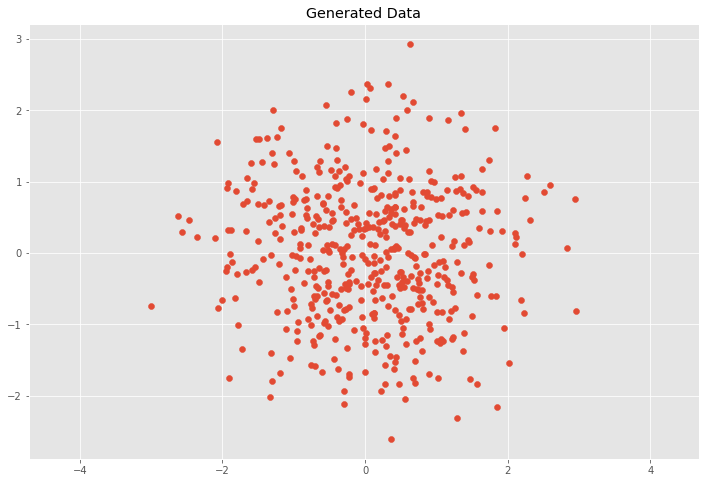
\includegraphics[scale=0.3]{uncorrelated.png}
   \caption{Uncorrelated Variables}
\end{figure}


This would mean that $X_1$ and $X_2$ are uncorrelated \footnote{Uncorrelated does not imply independent. See, e.g., \url{https://en.wikipedia.org/wiki/Normally_distributed_and_uncorrelated_does_not_imply_independent}}
and the covariance matrix $C$ is:
$$C = \left( \begin{array}{ccc}  \sigma^2 & 0 \\  0 & \sigma^2 \end{array} \right)$$

Next, we will look at how transformations affect our data and the covariance matrix $C$. We will transform our data with the following scaling matrix.
%$$S = \left( \begin{array}{ccc}  s_x & 0 \\  0 & s_y \end{array} \right)$$

$$S = \left( \begin{array}{ccc}  s_{1} & 0 \\  0 & s_{2} \end{array} \right)$$

where the transformation simply scales the $X_1$ and $X_2$ components by multiplying them by $s_{1}$ and $s_{2}$ respectively. Now the covariance matrix of our transformed data set will be:
%$$\frac{SX(SX)^T}{n-1}=S\frac{XX^T}{n-1}S^T=SCS^T=\left( \begin{array}{ccc}  (s_x\sigma_x)^2 & 0 \\  0 & (s_y\sigma_y)^2 \end{array} \right)$$.
$$\frac{SX(SX)^T}{n-1}=S\frac{XX^T}{n-1}S^T=SCS^T=\left( \begin{array}{ccc}  (s_{1}\sigma)^2 & 0 \\  0 & (s_{2}\sigma)^2 \end{array} \right)$$.

\begin{figure}[h!]
  \centering
    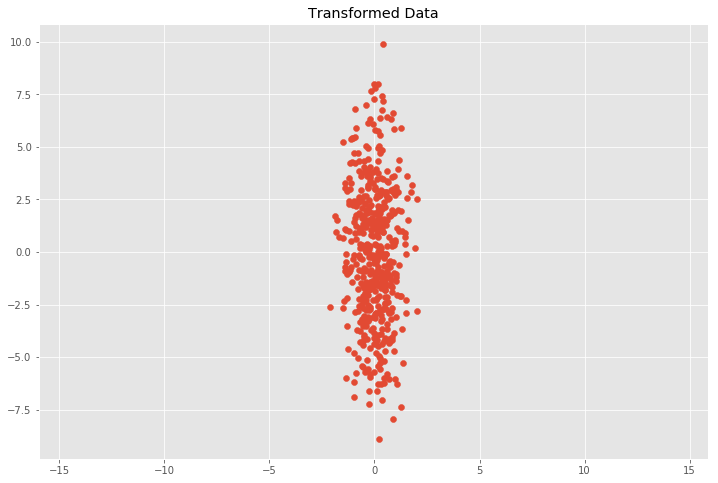
\includegraphics[scale=0.3]{uncorrelated_scaled.png}
   \caption{Uncorrelated Scaled Variables}
\end{figure}

Now we will apply a linear transformation in the form of a transformation matrix $T$ to the data set which will be composed of a two dimensional rotation matrix $R$ and the previous scaling matrix $S$ as follows: $$T = RS$$ where the rotation matrix $R$ is given by:
$$R = \left( \begin{array}{ccc}  \cos\theta  & -\sin\theta  \\  \sin\theta  & \cos\theta  \end{array} \right)$$

where $\theta$ is the rotation angle. The transformed data is then given by $RSX$ and the covariance matrix is

%$$\frac{YY^T}{n-1}=\frac{RSX(RSX)^T}{n-1}=RS\frac{XX^T}{n-1}S^TR^T=RSCS^TR^T=R\left( \begin{array}{ccc}  (s_x\sigma_x)^2 & 0 \\  0 & (s_y\sigma_y)^2 \end{array} \right)R^T$$.

$$\frac{RSX(RSX)^T}{n-1}=RS\frac{XX^T}{n-1}S^TR^T=RSCS^TR^T=R\left( \begin{array}{ccc}  (s_{1}\sigma)^2 & 0 \\  0 & (s_{2}\sigma)^2 \end{array} \right)R^T$$
$$=\sigma^2 \times \left( \begin{array}{ccc}  s^2_{1}\cos^2\theta +s^2_{2}\sin^2\theta  & \sin\theta \cos\theta (s^2_{1}- s^2_{2})\\  \sin\theta \cos\theta (s^2_{1}- s^2_{2}) & s^2_{1}\sin^2\theta +s^2_{2}\cos^2\theta  \end{array} \right)$$

Note that without applying an \emph{asymmetric} scaling, rotation alone would not be enough to create correlations since for $s_{1}= s_{2}$, the off-diagonal elements vanish.
\begin{figure}[h!]
  \centering
    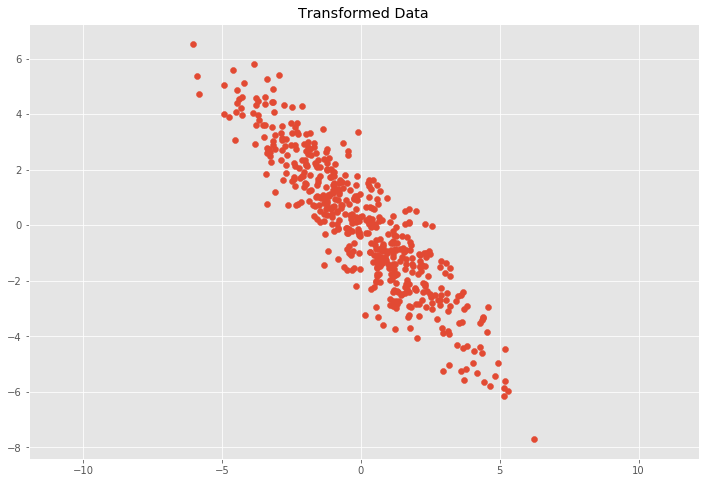
\includegraphics[scale=0.3]{correlated.png}
   \caption{Correlated Scaled Variables}
\end{figure}

As we can see now, the $x,y$ coordinate of each variable are not uncorrelated anymore. For example, if we know that the $x$ value of the sample is high, it is more likely that the $y$ value are low, and vice versa. Note, that $R$ is orthogonal, thus we got the eigenvalue decomposition (EVD) of the covariance matrix. Later in the course we are going to use some of the properties of the covariance matrix and its eigenvalue decomposition in the context of dimensionality reduction. 


\section{Probability Inequalities}
\subsection{Motivation and Background}
\footnote{This section based on lecture notes by Michal Moshkovitz and Alon Gonen} Probability inequalities are very useful in analyzing random processes. In particular, they are used to analyze machine learning algorithms. As we will see in class, in many learning tasks, we wish to estimate the expectation of some random variable
(e.g. the generalization error of a hypothesis) using the average of independently and identically distributed (i.i.d) random variables (e.g. the empirical loss of the same hypothesis). The law of large numbers states that the empirical average converges to the expected value. Probability inequalities provides us a means by which we can tell how good our estimates are when the sample is finite.

To be more concrete, consider the following task. Suppose that there is a bag containing red and blue balls. We would like to estimate the fraction $p$ of red balls in the bag. However, we are only
allowed to sample randomly from the bag with replacement. The straightforward strategy is to draw $n$ samples and predict
\[
\hat{p} = \frac{\# ~\text{of red balls}}{n}~.
\]
It is clear that $\E [\hat{p}] = p$. However, we might err due to the
fact that we get only limited information. Thus, we are
interested in an estimation with a certain additive error, 
$\epsilon$. Another obstacle is that since our process is random,
there is a probability that our sample doesn't represent the
distribution "well". Thus, we will further refine our objective. We will
be interested to guarantee with high probability that our estimator
has an additive error at most $\epsilon$.

More generally, concentration inequalities deal with the following fundamental
question: Given an accuracy parameter $\epsilon > 0$ and a confidence
parameter $\delta \in (0,1)$, how many samples are needed to guarantee that with probability of at least $1- \delta$, our estimate is within an additive error of at most $\epsilon$. The corresponding notion in supervised learning is called \emph{probably approximately correct (PAC)
learnability}. That is, we aim at constructing a learner whose
estimations are probably (with probability at least $1-\delta$)
approximately (within additive error of at most $\epsilon$) correct.

The exact formulation of the PAC framework will be given in the following lectures. Here, we will consider the well-known challenge of estimating the bias of a given coin. As we shall see, this moderate challenge reveals many of the ingredients of the PAC framework.

\subsection{Recap} \label{sec:recap}
We next recall Markov's and Chebyshev's inequalities and then apply both inequalities to derive concentration inequalities for averages.
\begin{theorem} \textbf{Markov's inequality:} For a nonnegative random
variable $X$ (i.e. $\text{Im}(X) \subseteq \reals_{\ge 0}$) with finite mean and a positive scalar $t$,
\[
\prob [X \geq t] \leq \frac{\mathbb{E}[X]}{t}~.
\]
\end{theorem}
\begin{proof}
Let $f(x)$ be the density function of $x$. Since $X$ is non-negative, we obtain
\begin{align*}
\E[X] &= \int_{x \in \reals} f(x) x \,dx \\&
= \int_{x = 0} ^t f(x) x\, dx + \int_{x =t} ^\infty f(x) x \, dx \\&
\ge \int_{x =t} ^\infty f(x) x \,dx \\&
\ge \int_{x =t} ^\infty f(x) t \, dx\\&
= t \cdot \int_{x =t} ^\infty f(x) \,dx \\&
=t \cdot \prob[X \ge t] ~.
\end{align*}
The desired inequality is obtained by dividing both sides by $t$.
\end{proof}
\begin{corollary} \label{cor:markovAve}
Let $X$ be a nonnegative random variable with finite mean. Denote its distribution by $\cD$. Let $X_1,\ldots,X_m$ be $m$ i.i.d. copies of $X$, i.e., $X_1,\ldots,X_m$ are i.i.d. random variables which are distributed according to $\cD$. Denote their average by $\overbar{X}=\frac{1}{m} \sum_{i=1} ^m X_i$. Finally, let $t>0$. Then
\[
\prob [\overbar{X} \geq t] \leq \frac{\mathbb{E}[X]}{t}~.
\]
\end{corollary}
\begin{proof}
By the linearity of the expectation,
\begin{align*}
\bE [\bar{X}] &= \bE \left[\frac{1}{m} \sum_{i=1} ^m X_i \right] \\&
= \frac{1}{m} \sum_{i=1} ^m \bE[X_i] \\&
= \frac{1}{m} \sum_{i=1} ^m \bE[X] \\&
= \bE[X]~.
\end{align*}
Applying Markov's inequality, we obtain the desired bound.
\end{proof}

Applying Markov inequality to the random variable $(X-\E[X])^2$, we obtain Chebyshev's inequality.
\begin{theorem} \textbf{Chebyshev's inequality:} For a random variable
  $X$ with finite mean and variance, and for every $t  > 0$,
\[
\prob[|X-\E [X]| \geq t] \leq \frac{Var[X]}{t^2}.
\]
\end{theorem}
\begin{proof}
Simply observe that $\prob[|X-\E [X]| \geq t] = \prob[(X-\E [X])^2 \geq t^2]$ and apply Markov's inequality.
\end{proof}
Unlike the expectation, the variance of the average of i.i.d. random variables is not equal to the variance of the original random variable. Concretely, for a random variable $X$ and $m$ i.i.d. copies of $X$, denoted $X_1,\ldots, X_m$, we have
\begin{align} \label{eq:varAve}
\rV \left[\frac{1}{m} \sum_{i=1} ^m X_i \right] &= \frac{1}{m^2} \rV \left[\sum_{i=1} ^m X_i \right] \notag \\&
= \frac{1}{m^2} \sum_{i=1} ^m \rV [X_i] \notag \\&
= \frac{1}{m^2} \sum_{i=1} ^m \rV [X] \notag \\&
= \frac{1}{m} \rV[X]~.
\end{align}
In particular, the variance of the average tends to zero when $m$ tends to infinity. This leads to a much better concentration inequality.
\begin{corollary} \label{cor:chebysevAve}
Let $X$ be a nonnegative random variable with finite variance and let $X_1,\ldots,X_m$ be $m$ i.i.d. copies of $X$. Denote their average by $\overbar{X}=\frac{1}{m} \sum_{i=1} ^m X_i$. Finally, let $t>0$. Then
\[
\prob [|\overbar{X}-\E [\overbar{X}]| \geq t] = \prob [|\overbar{X}-\E [X]| \geq t] \leq \frac{\rV[X]}{mt^2}~.
\]
\end{corollary}

For a positive integer $k$, the $k$-th \emph{moment} of a random variable $X$ is defined by $\bE[X^k]$. As we just saw, Markov's inequality exploits only information about the first moment, while Chebyshev's inequality exploits both the first and the second moments. Comparing the bounds in \corref{cor:markovAve} and \corref{cor:chebysevAve}, we see that using both the first and the second moments, we obtain better concentration inequalities than using only the first. We shall see soon that more generally, the more moments we use, the better the bounds we get.


\subsection{Coin Prediction}  \label{sec:basicConcentration}
Let us formulate the problem of estimating the bias of a
coin (in short, coin prediction)\footnote{We take this opportunity to recall some basic notions from probability theory}. Formally, a coin is a Bernoulli random variable $Z$ with a bias $p - 1/2$ ('bias' is defined here as the \textit{deviation} from $p=1/2$, where $p$ is the probability to obtain ``heads''). 
%The probability space which is associated with $Z$ is the triplet $(\Omega ,\prob )$, where the sample space $\Omega$ equals $\{H,T\}$,  $$\prod\{1\}]=p~,~\cD[\{0\}]=1-p~. $$Once we defined $\cD(\{1\})$ and $\cD(\{0\})$, the values of $\cD$ on other events are determined by combining the fact that $\cD$ is additive (for disjoints subsets $E,F \in \cF$, we have $\cD(E \cup F)=\cD(E) + \cD(F)$) with the fact that $\cD(\Omega)=1$.
The random variable $Z$ is simply a function from $\Omega$ to $\{0,1\}$. Let $Z_1,
\ldots, Z_m$ be a sequence of independent and identically distributed
(i.i.d.) random variables according to the distribution $\cD_Z$ (that
is, each of the $Z_i$ has the same distribution as $Z$, and all of the
$Z_i$ are mutually independent). Denote the random sequence  (a.k.a. sample)
$(Z_1,\ldots, Z_m)$ by $S$, where $|S|=m$. The distribution which is associated with $S$ is denoted by $\cD_Z ^m$ (or simply by $\cD^m$).

The input of a \emph{learning algorithm} $A$ for the task of coin prediction consists of a random sequence $S$ which is drawn according to
$\cD^m$. Based on this input, the algorithm has to predict the value of $p$. We denote this prediction, (that is, the output of the algorithm) by $A(S)$ or simply by $\hat{p}$. Clearly, the drawn sequence can not fully describe the distribution. Hence, we introduce an \emph{accuracy} parameter $\epsilon>0$, and allow $\hat{p}$ to deviate from $p$ by at most $\epsilon$. Furthermore, there is always a chance that the drawn sequence would be highly non-representative, so it is impossible to obtain a guarantee that holds with absolute certainty. Hence, we introduce a \emph{confidence} parameter $\delta>0$, and allow that the event $B:=\{s : |\hat{p}-p|>\epsilon\}$ occur with probability at
most $\delta$. More formally:

\begin{definition}  \label{def:sampleCoin}
A mistake-bound learning algorithm $A$ for the task of (batch) coin prediction is a function $\hat{p}(S)$
where $S\in \bigcup_{m=1} ^\infty \{0,1\}^m$ and $\hat{p}(S)\in [0,1]$ which satisfies the following condition:
 
For any $0\le \epsilon,\delta\le 1$, there exists a non-negative integer $m_A(\epsilon,\delta)$ such that, 
 if a sequence $S$ of $m$ numbers, where $m\ge m_A$, is generated according to $\cD^m_p$, (that is, $\cD^m$ with parameter $p$, which is added temporarily here as a subscript but omitted later on) then the probability that the algorithm's output $\hat{p}(S)$ will not be in $[p-\epsilon,p+\epsilon]$ is bounded by:
$$ \cD^{m}_p \left[ |\hat{p}-p| > \epsilon\right] <  \delta,$$
\textbf{for any $0\le p\le 1$,} and if a sequence $S$ of $m$ numbers, where $m < m_A$, is generated, \textbf{there exist a $p$}, with $0\le p\le 1$ such that:
$$ \cD^{m}_p \left[ |\hat{p}-p| >  \epsilon \right] > \delta$$

The function $m_A(\epsilon,\delta)$: $\left[0,1\right]\times \left[0,1\right]\rightarrow \mathbb{N}$ is called the \emph{sample complexity} of the learning algorithm $A$.

% More generally: the sample complexity of a machine learning algorithm represents the number of training-samples that it needs in order to successfully learn a target function.
\end{definition}

The first condition means that, no matter what $p$ is, it is enough to draw $m_A$ samples (i.e., to flip the coin $m_A$ times) in order to know $p$, with a certainty of $1-\delta$ and an accuracy of $\pm \epsilon$. The second conditions means that, at least for some values of $p$, drawing $m_A(\epsilon,\delta)-1$ samples would \textit{not} be enough for that.

\textbf{Note about the confidence requirement}: In the above definition the confidence requirement must hold \emph{independently of the procedure by which the coins are provided}, that is, independently of the way $p$ is chosen. It does not matter if, for example, the coin is randomly drawn from a pile of coins where most coins are approximately fair (most of their $p$'s are close to $1/2$) or where most are faked in a specific way, (their $p$'s are concentrated around, say, $\frac{1}{4}$ ),  or where all $p$'s are equally probable. 

Another way to think of the sample complexity is the following. Consider all possible sequences, $S$, of $m$ 0's and 1's. For each value of $p$, each of these sequences has a different probability to occur. Each $S$ can be labeled as 'good' ('typical') or 'bad'('atypical'), 'good' means that $m \cdot \hat{p}(S)$ is between $m(p-\epsilon)$ and $m(p+\epsilon)$ and 'bad' otherwise (Note that,  even for the same coin,  if  $S$ is good with respect to algorithm $A_1(S)$ it may still be bad with respect to another algorithm $A_2(S),$  if $\hat{p}_1(S)\ne \hat{p}_2(S)$.) Given a coin, let us denote the smallest $m$ for which the  total sum of the probabilities of all the good sequences is at least $1-\delta$, by $m_A^{(p)}(\epsilon,\delta)$. We can think of $m_A^{(p)}$ as the \emph{coin-specific} sample complexity. The algorithm sample complexity $m_A(\epsilon,\delta)$ is the maximal number among the coin-specific sample complexities, that is: $m_A(\epsilon,\delta) = \max_{p}(m_A^{(p)}(\epsilon,\delta))$.

%The term `approximately' in PAC stems from the fact that we only require that $\hat{p}$ approximates $p$ to an accuracy $\epsilon$. The term `probably' in PAC comes from the fact that we are satisfied whenever $\hat{p}$ satisfies the accuracy requirements with probability at least$1-\delta$.

Given an i.i.d. random sample $S=(z_1, \ldots, z_m)$, a reasonable
estimate of $p$ is the empirical proportion of heads (ones), namely
$\hat{p}=\frac{1}{m} \sum_{i=1} ^m z_m$. The first basic property of
this average is that its expected value equals $p$. This follows by
the linearity of expectation as follows:
\[
\bE \left [\frac{1}{m} \sum_{i=1} ^m Z_i \right] = \frac{1}{m} \sum_{i=1} ^m
\bE[Z_i] = \frac{1}{m} \cdot m \cdot p = p~.
\]
We say in this case that $\hat{p}$ forms an \emph{unbiased estimate}
of $p$. What can we say about the quality of $\hat{p}$ as an estimate
of $p$? In other words, how tightly $\hat{p}$ is concentrated around
its expectation? To answer this question, we can use concentration inequalities.\\

\noindent \textbf{First attempt: Markov's inequality: }

For a direct application of Markov's inequality we take  $|\hat{p}-p|$ as our RV  (note that $\hat{p}-p$ is not a positive RV and therefore cannot be used in Markov's inequality). We then need to calculate $\frac{1}{\epsilon}\bE[|\hat{p}-p|]$ and extract its dependence on the sample size $m$.
Since we are going to get much better bounds below, here we only state the result (and leave the calculation as a challange exercise):
$$
\cD^m \left[|\hat{p}-p| \geq \epsilon \right]  \le \frac{1}{\sqrt{4m\epsilon^2}}
$$
This implies that the sample complexity of coin prediction is bounded above by
$m(\epsilon,\delta) \le \left \lceil \frac{1}{4\epsilon^2} \cdot
  \frac{1}{\delta^2} \right \rceil$.
  (You can verify by substituting $m=\frac{1}{4\epsilon^2}\cdot
  \frac{1}{\delta^2}$ in the bound)

\vspace{5mm}

\begin{exercise}[Markov's inequality]
Prove that:  $\cD^m \left[|\hat{p}-p| \geq \epsilon \right]  \le \frac{1}{\sqrt{4m\epsilon^2}}.$ 
\end{exercise}

\begin{itemize}
	\item Hint: Show that for any RV $h$ with $\bE(h)=0$ :
$$\bE(|h|) \le \sqrt{ Var(h)}$$
and then apply this result to the RHS of Markov's inequality.

	\item Use the above to obtain a bound over the sample complexity and compare it to the one obtained from the Chebyshev's inequality.
\end{itemize} 
\color{black}

\noindent \textbf{Second attempt: Chebyshev's inequality: }
The variance of a Bernoulli random variable is $p(1-p) \le 1/4$. Applying \corref{cor:chebysevAve}, we obtain that
$$ \cD^m [|\hat{p}-p| \ge \epsilon] = \cD^m[|\hat{p}-\mathbb{E} [\hat{p}]| \ge \epsilon] \le \frac{Var[Z]}{m\epsilon^2} \le \frac{1}{4m \epsilon ^2}$$

The bound obtained using Chebyshev's inequality tends to zero as $\frac{1}{m}$ while the one obtained from Markov's inequality tends to zero as $\frac{1}{\sqrt{m}}$.
This fact enables us to obtain a better bound for the sample complexity:

\begin{corollary}  \label{cor:basicConcentration}
The sample complexity of coin prediction is bounded above by
$m(\epsilon,\delta) \le \left \lceil \frac{1}{4\epsilon^2} \cdot
  \frac{1}{\delta} \right \rceil$.
  (You can verify by substituting $m=\frac{1}{4\epsilon^2} \cdot
  \frac{1}{\delta}$ in the bound)
\end{corollary}


\color{black}


A natural question which arises is whether the obtained bound is optimal (tight). There is a good reason to suspect that this bound is not optimal; When we applied Markov's or Chebyshev's inequality, we did not exploit the fact that our RV's are bounded (between $0$ and $1$).  Indeed, in the next section we prove a much better bound \footnote{Which is tight, although we will not prove that}. For this end, we will introduce Hoeffding's inequality for the average of independent and bounded random variables. This inequality will give us exponential (instead of polynomial!) convergence in terms of the sample size $m$.

\subsubsection{Hoeffding's Inequality}
\begin{theorem}[Hoeffding's inequality]
Let $X_1, \ldots X_m$ be independent and bounded random variables with $a_i \leq X_i \leq b_i$. Let $\bar{X} = \frac{1}{m} \sum_{i=1} ^m X_i$. Then,
\[
\prob [ |\bar{X} - \E[\bar{X}]| \geq \epsilon ] \leq 2 \exp \left( \frac{-2m^2 \epsilon^2}{\sum _{i =1} ^m (b_i-a_i)^2} \right)
\]
\end{theorem}
\begin{corollary}
Let $X_1, \ldots X_m$ be a sequence of i.i.d. (independent \textbf{and} identically distributed) and bounded with $a \leq X_i \leq b$ (same $a, b$ for all $X_i$'s). Let $\bar{X} = \frac{1}{m} \sum_{i=1} ^m X_i$ and let $\mu = \E[X_i]$. Then,
\[
\prob [|\bar{X} - \mu| \geq \epsilon] \leq 2 \exp \left( \frac{-2 m \epsilon^2}{(b-a)^2} \right)
\]
\end{corollary}

\subsubsection{Coin Prediction Revisited}
Lets apply Hoeffding's inequality for the case of coin prediction which was discussed above. For a sample of size $m$, we obtain
\[
\cD^m [|\hat{p}-p| \ge \epsilon ]\leq  2 \exp(-2 m \epsilon ^2)~.
\]
Indeed, we achieve an exponential improvement (in terms of $\delta$).
\begin{corollary}  \label{cor:basicConcentration}
The sample complexity of coin prediction is bounded above by
$m(\epsilon,\delta) \le \left \lceil \frac{1}{2\epsilon^2} \cdot
  \log(\frac{2}{\delta}) \right \rceil$.
  (You can verify by substituting $m=\frac{1}{2\epsilon^2} \cdot
  \log(\frac{2}{\delta})$ in the bound)
\end{corollary}

